\documentclass[11pt,a4paper]{article}
\usepackage[T1]{fontenc}
\usepackage[utf8]{inputenc}
\usepackage{lmodern}
\usepackage{amsmath,amssymb,amsthm,mathtools,mathrsfs}
\usepackage{graphicx,float,xcolor,multicol}
\usepackage[shortlabels]{enumitem}
\usepackage[margin=27mm]{geometry}
\usepackage{microtype,needspace,placeins}
\usepackage{tikz,tikz-cd}
\usetikzlibrary{arrows.meta,calc,positioning,patterns,decorations.pathreplacing}
\usepackage[colorlinks=true,linkcolor=teal,urlcolor=teal,citecolor=teal]{hyperref}
\setlength{\parindent}{0pt}
\setlength{\parskip}{.6em}
\setcounter{secnumdepth}{0}
\allowdisplaybreaks
\raggedbottom
\providecommand{\cross}{\times}
\DeclareUnicodeCharacter{2020}{\ensuremath{\dagger}}
\DeclareMathOperator{\supp}{supp}
\DeclareMathOperator*{\esssup}{ess\,sup}
\providecommand{\chapter}{\section}
\newenvironment{tool}[2]{\subsection*{Tool #1 --- #2}}{}
\newcommand{\ToolRef}[1]{Tool #1}
\newcommand{\FigureTag}[2]{\textit{Figure #1}}
\newcommand{\Result}[1]{\subsection*{#1}}
\newcommand{\Application}[1]{\subsubsection*{Application\if\relax\detokenize{#1}\relax\else\space--- #1\fi}}
\newcommand{\ProofHeading}{\par\textit{Proof.}\space}
\newcommand{\ProofOf}[1]{\par\textit{Proof of #1.}\space}
\newcommand{\RemarkHeading}{\par\textbf{Remark.}\space}
\newcommand{\NoteHeading}{\par\textbf{Note.}\space}
\newcommand{\ExerciseHeading}{\par\textbf{Exercise.}\space}

% Rendering support only; mathematical text is in each independent post.
\usepackage{booktabs,array,longtable}
\definecolor{HandoutBlue}{HTML}{2F6690}
\definecolor{HandoutNavy}{HTML}{17365D}
\newtheorem{theorem}{Theorem}
\newtheorem{lemma}[theorem]{Lemma}
\newtheorem{proposition}[theorem]{Proposition}
\newtheorem{corollary}[theorem]{Corollary}
\newtheorem{conjecture}[theorem]{Conjecture}
\newtheorem{definition}{Definition}
\newtheorem{example}{Example}
\newtheorem{namedtoolcounter}{Tool}
\newenvironment{namedtool}[1]{\begin{namedtoolcounter}[#1]}{\end{namedtoolcounter}}
\newtheorem*{claim}{Claim}
\newtheorem*{remark}{Remark}
\newtheorem*{exercise}{Exercise}
\newtheorem*{question}{Question}
\newtheorem*{observation}{Observation}
\newcommand{\SourceChapter}[2]{\section*{#2}}
\newcommand{\Lecture}[2]{\section*{Lecture #1: #2}}
\newcommand{\unclear}[1]{\textit{[unclear: #1]}}
\newcommand{\sourcegap}{\textit{[unfinished in the source]}}
\DeclareMathOperator{\dist}{dist}
\DeclareMathOperator{\id}{id}
\DeclareMathOperator{\Hol}{Hol}
\DeclareMathOperator{\Per}{Per}
\DeclareMathOperator{\Fix}{Fix}
\DeclareMathOperator{\diam}{diam}
\DeclareMathOperator{\Var}{Var}
\DeclareMathOperator{\Leb}{Leb}
\DeclareMathOperator{\Hom}{Hom}
\DeclareMathOperator{\End}{End}
\DeclareMathOperator{\Ann}{Ann}
\DeclareMathOperator{\Spec}{Spec}
\DeclareMathOperator{\Max}{Max}
\DeclareMathOperator{\Ob}{Ob}
\DeclareMathOperator{\Tor}{Tor}
\DeclareMathOperator{\Ass}{Ass}
\DeclareMathOperator{\Mor}{Mor}
\DeclareMathOperator{\Fun}{Fun}
\DeclareMathOperator{\Nat}{Nat}
\DeclareMathOperator{\Cone}{Cone}
\DeclareMathOperator{\MCG}{MCG}
\DeclareMathOperator{\Aut}{Aut}
\DeclareMathOperator{\Deck}{Deck}
\DeclareMathOperator{\SL}{SL}
\DeclareMathOperator{\PSL}{PSL}
\DeclareMathOperator{\Area}{Area}
\DeclareMathOperator{\im}{im}
\DeclareMathOperator{\PSh}{PSh}
\newcommand{\CRing}{\mathsf{CRings}}
\newcommand{\AMod}{A\text{-}\mathsf{Mod}}
\newcommand{\Ab}{\mathsf{Ab}}
\newcommand{\Z}{\mathbb Z}
\newcommand{\Q}{\mathbb Q}
\newcommand{\R}{\mathbb R}
\newcommand{\C}{\mathbb C}
\newcommand{\N}{\mathbb N}
\newcommand{\kk}{\mathbb k}
\renewcommand{\aa}{\mathfrak a}
\newcommand{\bb}{\mathfrak b}
\newcommand{\pp}{\mathfrak p}
\newcommand{\qq}{\mathfrak q}
\newcommand{\mm}{\mathfrak m}
\newcommand{\nn}{\mathfrak n}
\newcommand{\rad}{\mathrm r}
\newcommand{\cat}[1]{\mathsf{#1}}
\setcounter{secnumdepth}{0}
\allowdisplaybreaks

\graphicspath{{figures/complex-dynamics-notes/}}
\begin{document}
\section*{The Chain Rule and Complex Dilatation}
% BLOG-CONTENT-BEGIN
Given a manifold \(M\), local coordinates \((U,x_1,\ldots,x_n)\) tell us the whereabouts of points in \(U\). Directions, however, cannot be represented in terms of the \(x_i\). That luxury is available only in Euclidean spaces such as \(\mathbb R^n\), where \(x_i\) is projection onto the \(i\)-th coordinate. There, moving in the \(i\)-th coordinate means moving in the direction \(x_i\). To say something similar on a manifold, we introduce \emph{tangent spaces}.

If a path allows us to associate a direction coherently at every point, for instance a smooth curve \(\gamma:[0,1]\to M\), then \(\gamma'(t)\) is a point of \(T_{\gamma(t)}M\cong\mathbb R^n\).
\begin{figure}[H]\centering
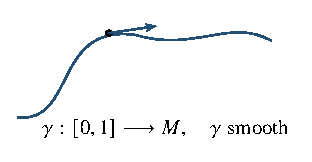
\includegraphics[width=.48\textwidth]{cd9-fig-01.pdf}
\FigureTag{CD9.1}{fig:cd9-01}
\end{figure}
By identifying \(\gamma'(t)\) with a vector in \(\mathbb R^n\), one can associate an \emph{infinitesimal} direction. Changing direction amounts to changing one's path at a given point \(P\), as below. Thus tangent spaces allow us to navigate a manifold.
\begin{figure}[H]\centering
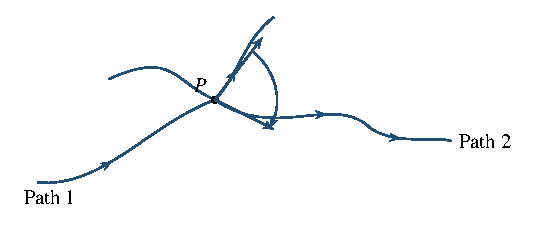
\includegraphics[width=.7\textwidth]{cd9-fig-02.pdf}
\FigureTag{CD9.2}{fig:cd9-02}
\end{figure}

% Source page 2
As in \(\mathbb R^n\), moving in the \(i\)-th coordinate on \(M\), or moving along \(x_i\), means moving only along \(x_i\): the rate of change along \(x_j\), for \(j\ne i\), is zero. Thus
\(\{\left.\partial/\partial x_i\right|_p\}_{i=1}^n\) is an appropriate basis for \(T_pM\).

If the coordinates change from \((U,x_1,\ldots,x_n)\) to \((U,y_1,\ldots,y_n)\), then \(T_pM\), \(p\in U\), has two bases. Write
\[
\frac{\partial}{\partial x_i}=\sum_{j=1}^n a_j\frac{\partial}{\partial y_j}.
\]
The simplest way to find this change of basis is to evaluate both sides on \(y_k\). This gives \(a_k=\partial y_k/\partial x_i\); the matrix is
\(\bigl(\partial y_k/\partial x_i\bigr)_{1\le i,k\le n}\).
Changing coordinates is therefore no trouble: this matrix acts like a dictionary!

% Source page 3
The same can be done for complex manifolds. On a real or complex manifold, the directions along \(\gamma(t)\) are
\[
\gamma'(t)=\sum_{i=1}^n\gamma_i'(t)
\left.\frac{\partial}{\partial x_i}\right|_{\gamma(t)}\in TM,
\]
where \(TM\) is the tangent bundle.

There is a dual notion to navigation on a manifold: \emph{obstruction}. Suppose the curve moves in the direction
\[
\gamma_1'(t)\left.\frac{\partial}{\partial x_1}\right|_{\gamma(t)}
+\gamma_2'(t)\left.\frac{\partial}{\partial x_2}\right|_{\gamma(t)}.
\]
To know what obstructs \(\gamma\) from moving purely in the \(x_1\)-direction, we must retrieve the extra luggage
\(\gamma_2'(t)\left.\partial/\partial x_2\right|_{\gamma(t)}\), which is \emph{misdirecting} its flow.
To study flow, or navigation, we looked naturally at functions \(\gamma:\mathbb R\to M\). To study its dual, obstruction, focus instead on \(f:M\to\mathbb R\), \(f\in C^\infty(M)\).

Define the differential of \(f\) at \(p\) by \(df_p(v)=v_p(f)\), where \(v\in T_pM\). Thus \(df_p\) is a covector: it is a linear functional on \(T_pM\), given by evaluation. The family \(\{dx_i\}_{i=1}^n\) is a smooth coframe on \(U\), so
\[
df_p=a_i(p)(dx_i)|_p,\qquad
a_i(p)=df_p\left(\left.\frac{\partial}{\partial x_i}\right|_p\right)
=\left.\frac{\partial f}{\partial x_i}\right|_p.
\]
Consequently \(df_p=\left.(\frac{\partial f}{\partial x_i}\,dx_i)\right|_p\).

% Source page 4
Since \(\partial f(p)/\partial x_i\) is smooth, \(df\) is a smooth covector field. Set \(f=x_2\). Then
\[
df_{\gamma(t)}\bigl(\gamma'(t)\bigr)
=\gamma_1'(t)\left.\frac{\partial x_2}{\partial x_1}\right|_{\gamma(t)}
+\gamma_2'(t)\left.\frac{\partial x_2}{\partial x_2}\right|_{\gamma(t)}
=\gamma_2'(t).
\]
The obstruction to the flow \(\gamma(t)\) along \(x_2\) is therefore given by
\((dx_2)_{\gamma(t)}(\gamma'(t))\), and \(df_p\in T_p^*M\), the dual tangent space.
Flows and obstructions can be discussed using the two bundles \(TM\) and \(T^*M\) hovering over the manifold.

Let us now combine flow and obstruction. For a smooth curve \(\gamma:J\to M\) and \(f:M\to\mathbb R\), \(f\in C^\infty(M)\), one has
\[
(f\circ\gamma)'(t)=df_{\gamma(t)}\bigl(\gamma'(t)\bigr).
\]
In plain English, the obstruction to \(\gamma(t)\) along \(f\) is the same as the flow of \(f\circ\gamma\). In modest terms, the chain rule chains together flows and obstructions in a very intricate manner! Let us see what more it can offer.

% Source page 5
For \(f:\mathbb C\to\mathbb C\), viewed as a map \(\mathbb R^2\to\mathbb R^2\), we know
\(df=f_x\,dx+f_y\,dy\). Alternatively,
\[
df=f_z\,dz+f_{\bar z}\,d\bar z,\qquad
dz=dx+i\,dy,\quad d\bar z=dx-i\,dy,
\]
where
\[
\partial_z:=\frac{\partial}{\partial z}
=\frac12\left(\frac{\partial}{\partial x}-i\frac{\partial}{\partial y}\right),
\qquad
\partial_{\bar z}:=\frac{\partial}{\partial\bar z}
=\frac12\left(\frac{\partial}{\partial x}+i\frac{\partial}{\partial y}\right).
\]
As \(df\) acts linearly pointwise, focus on one point rather than on the smooth covector field. For \(df_z:T_z\mathbb C\to T_{f(z)}\mathbb C\), set
\[
\mu_f=\frac{\partial_{\bar z}f}{\partial_zf},\qquad
\alpha=\arg(\partial_zf),\qquad \theta=\arg\mu_f,
\]
assuming that \(\mu_f\) is defined and \(|\mu_f|<1\). Then
\[
df_z(\omega)=e^{i\alpha}|\partial_zf|
\bigl(\omega+|\mu_f|e^{i\theta}\bar\omega\bigr).
\]
The vectors \(e^{i\theta/2}\) and \(e^{i(\pi+\theta)/2}\) are eigenvectors of \(df_z/e^{i\alpha}\). Linear maps pull ellipses back to ellipses, giving the following picture.
\begin{figure}[H]\centering
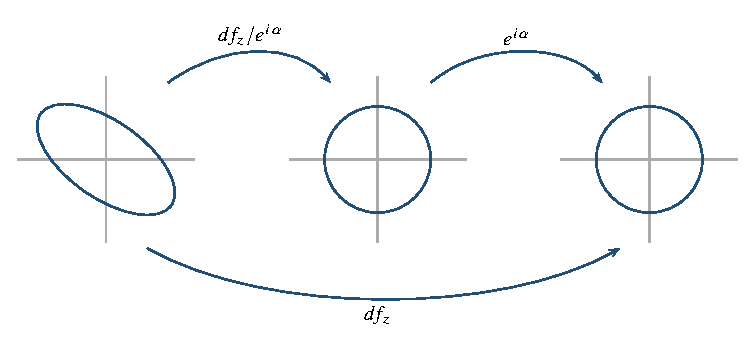
\includegraphics[width=.85\textwidth]{cd9-fig-03.pdf}
\FigureTag{CD9.3}{fig:cd9-03}
\end{figure}

% Source page 6
Before proceeding, observe that
\[
d(f\circ g)_z=df_{g(z)}\circ dg_z
=(f_z\circ g)\,dg_z+(f_{\bar z}\circ g)\,d\bar g_z.
\]
Expanding gives
\[
\begin{aligned}
d(f\circ g)_z={}&
\bigl[(f_z\circ g)g_z+(f_{\bar z}\circ g)\overline{g_{\bar z}}\bigr]\,dz\\
&+\bigl[(f_z\circ g)g_{\bar z}
+(f_{\bar z}\circ g)\overline{g_z}\bigr]\,d\bar z.
\end{aligned}
\]
From this simple composition of linear maps one obtains the chain rule for the Wirtinger derivatives:
\[
\begin{aligned}
\partial_z(f\circ g)&=(f_z\circ g)g_z+(f_{\bar z}\circ g)\overline{g_{\bar z}},\\
\partial_{\bar z}(f\circ g)&=(f_z\circ g)g_{\bar z}+(f_{\bar z}\circ g)\overline{g_z}.
\end{aligned}
\]

% Source page 7
The coefficient \(\mu_f(z)\) captures the shape of the ellipse pulled back from \(T_{f(z)}\mathbb C\). Its ratio of major to minor axes is
\[
K_f=\frac{1+|\mu_f|}{1-|\mu_f|}.
\]
% BLOG-CONTENT-END
\end{document}
